\documentclass{memoir}
\usepackage{fdvs-style}
\usepackage{fdvs-style-operators}

\begin{document}

\setcounter{section}{12}

\section{Dual Spaces}

\begin{dfn}[Dual Space]
Given a vector space $V$, we define the \emph{dual space} of $V$ to be the vector space $\Dual{V} = \Hom{V}{F}$. If $\varphi : V \rightarrow W$ is a linear transformation, then the map $\Dual{\varphi} : \Dual{W} \rightarrow \Dual{V}$ given by $\Dual{\varphi}(\mu) = \mu \circ \varphi$ is called the \emph{dual} of $\varphi$.
\end{dfn}

\begin{prp} \mbox{}
\begin{enumerate*}
\item $\Dual{1_V} = 1_{\Dual{V}}$
\item $\Dual{\psi \circ \varphi} = \Dual{\varphi} \circ \Dual{\psi}$
\end{enumerate*}
\end{prp}

\begin{proof} \mbox{}
\begin{enumerate*}
\item If $\mu \in \Dual{V}$, then \[ \Dual{1_V}(\mu) = \mu \circ 1_V = \mu = 1_{\Dual{V}}(\mu) \] as needed.
\item If $\mu \in \Dual{V}$, then \[ \left(\Dual{\varphi \circ \psi}\right)(\mu) = \mu \circ \varphi \circ \psi = \Dual{\psi}(\mu \circ \varphi) = \Dual{\psi}(\Dual{\varphi}(\mu)) = \left(\Dual{\psi} \circ \Dual{\varphi}\right)(\mu) \] as needed. \qedhere
\end{enumerate*}
\end{proof}

\begin{prp} \mbox{}
\begin{enumerate*}
\item If $\varphi$ is injective, then $\Dual{\varphi}$ is surjective.
\item If $\varphi$ is surjective, then $\Dual{\varphi}$ is injective.
\end{enumerate*}
\end{prp}

\begin{proof}
Remember that $\varphi$ is injective if and only if there is a linear transformation $\psi$ such that $\psi \circ \varphi = 1_V$, and is surjective if and only if there is a $\psi$ such that $\varphi \circ \psi = 1_W$. If $\varphi$ is injective, then we have \[ \Dual{\varphi} \circ \Dual{\psi} = \Dual{\psi \circ \varphi} = \Dual{1_V} = 1_{\Dual{V}} \] so that $\Dual{\varphi}$ is surjective. Likewise for (ii).
\end{proof}

\begin{dfn}
Given a subset $S \subseteq V$, the \emph{annihilator} of $S$ in $\Dual{V}$ is the subset $\Ann*{S} = \{ \varphi \mid S \subseteq \Ker*{\varphi} \} \subseteq \Dual{V}$.
\end{dfn}

\begin{prp}
Let $S \subseteq V$ be a subset and $W \subseteq V$ a subspace. Then we have the following.

\begin{inparaenum}
\item $\Ann*{S}$ is a subspace of $\Dual{V}$. \hfill
\item $\Dual{W} \cong \Dual{V}/\Ann*{W}$ \hfill
\item $\Dual{V/W} \cong \Ann*{W}$
\end{inparaenum}
\end{prp}

\begin{proof} \mbox{}
Exercise.
\end{proof}

\begin{prp}
Fix a basis $\mathcal{B} \subseteq V$. For each $b \in \mathcal{B}$, let $\Dual{b} \in \Dual{V}$ be the unique linear transformation such that $\Dual{b}(e) = 1$ if $e = b$ and $0$ otherwise for all $e \in \mathcal{B}$. Then
\begin{enumerate*}
\item The set $\Dual{\mathcal{B}} = \{\Dual{b} \mid b \in \mathcal{B}\}$ is independent in $\Dual{V}$.
\item The linear mapping $d_\mathcal{B} : V \rightarrow \Dual{V}$ such that $b \mapsto \Dual{b}$ is injective.
\item If $V$ is finite dimensional, then $\Dual{\mathcal{B}}$ is a basis of $\Dual{V}$, which we call the \emph{dual} of $\mathcal{B}$.
\end{enumerate*}
\end{prp}

\begin{proof} \mbox{}
\begin{enumerate*}
\item Suppose we have $\alpha_i \in F$ and $\Dual{b_i} \in \Dual{\mathcal{B}}$ such that $\sum_{i=1}^k \alpha_i \Dual{b_i} = 0$. That is, this linear combination is the zero mapping from $V$ to $F$. In particular, for each $b_t$ where $t \in \intrange{1}{k}$, we have \[ 0 = 0(b_t) = \left(\sum_{i=1}^k \alpha_i \Dual{b_i}\right)(b_t) = \sum_{i=1}^k \alpha_i \Dual{b_i}(b_t) = \alpha_t. \] So in fact $\Dual{\mathcal{B}}$ is independent.
\item The image of the basis $\mathcal{B} \subseteq V$ is independent.
\item It suffices to show that $\Dual{\mathcal{B}}$ is a generating set of $\Dual{V}$. But clearly we have, for each $\mu \in \Dual{V}$, \[ \mu = \sum_{i=1}^n \mu(b_i) \Dual{b_i} \] as needed. \qedhere
\end{enumerate*}
\end{proof}

\begin{prp}
Let $V$ and $W$ be finite dimensional with ordered bases $\mathcal{B}$ and $\mathcal{E}$, respectively, and let $\varphi : V \rightarrow W$ be a linear transformation. Then \[ [\Dual{\varphi}]^{\Dual{\mathcal{E}}}_{\Dual{\mathcal{B}}} = \left([\varphi]^\mathcal{B}_\mathcal{E}\right)^\mathsf{T}. \]
\end{prp}

\begin{proof}
Let us write $\mathcal{B} = \{ b_1, \ldots, b_m \}$ and $\mathcal{E} = \{e_1, \ldots, e_n \}$. For each $j \in \intrange{1}{m}$ and each $i \in \intrange{1}{n}$, write \[ \varphi(b_j) = \sum_{k=1}^n \mu_{k,j} e_k \quad \mathrm{and} \quad \Dual{\varphi}(\Dual{e_i}) = \sum_{\ell=1}^m \eta_{\ell,i} \Dual{b_\ell}, \] so that (by definition) \[ [\varphi]^\mathcal{B}_\mathcal{E} = [\mu_{k,j}]_{k=1,j=1}^{n,m} \quad \mathrm{and} \quad [\Dual{\varphi}]^{\Dual{\mathcal{E}}}_{\Dual{\mathcal{B}}} = [\eta_{\ell,i}]_{\ell=1,i=1}^{m,n}. \] We will now consider the value of $\Dual{\varphi}(\Dual{e_i})(b_j)$ for each $i \in \intrange{1}{n}$ and $j \in \intrange{1}{m}$. On one hand, we have \[ \Dual{\varphi}(\Dual{e_i})(b_j) = \left( \sum_{\ell=1}^m \eta_{\ell,i} \Dual{b_\ell} \right)(b_j) = \sum_{\ell=1}^m \eta_{\ell,i} \Dual{b_\ell}(b_j) = \eta_{j,i}. \] On the other hand, we have \[ \Dual{\varphi}(\Dual{e_i})(b_j) = (\Dual{e_i} \circ \varphi)(b_j) = \Dual{e_i}\left( \varphi(b_j) \right) = \Dual{e_i}\left( \sum_{k=1}^n \mu_{k,j} e_k \right) = \sum_{k=1}^n \mu_{k,j} \Dual{e_i}(e_k) = \mu_{i,j}. \] So, by definition, \[ [\Dual{\varphi}]^{\Dual{\mathcal{E}}}_{\Dual{\mathcal{B}}} = \left([\varphi]^\mathcal{B}_\mathcal{E}\right)^\mathsf{T}. \qedhere \]
\end{proof}

\begin{prp}
Let $V$ be a vector space. 
\begin{enumerate}
\item Given $v \in V$, we define $\eta_V(v) : \Dual{V} \rightarrow F$ by $\eta_V(v)(\mu) = \mu(v)$. Then $\eta_V(v)$ is linear, so that in fact $\eta_V(v) \in \Dual{\Dual{V}}$. Moreover, $\eta_V : V \rightarrow \Dual{\Dual{V}}$ is linear.
\item If $\varphi : V \rightarrow W$ is a linear transformation, then $\Dual{\Dual{\varphi}} \circ \eta_V = \eta_W \circ \varphi$. That is, the following diagram commutes.

\begin{center}
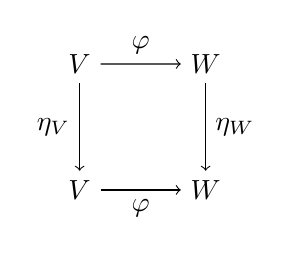
\begin{tikzpicture}[scale=0.4]
\node (V) at (0,4) {$V$};
\node (W) at (4,4) {$W$};
\node (DDV) at (0,0) {$\Dual{\Dual{V}}$};
\node (DDW) at (4,0) {$\Dual{\Dual{W}}$};
\draw[->] (V) edge node [above] {$\varphi$} (W);
\draw[->] (V) edge node [left] {$\eta_V$} (DDV);
\draw[->] (W) edge node [right] {$\eta_W$} (DDW);
\draw[->] (DDV) edge node [below] {$\Dual{\Dual{\varphi}}$} (DDW);
\end{tikzpicture}
\end{center}
\end{enumerate}
\end{prp}

\begin{proof} \mbox{}
\begin{enumerate*}
\item Exercise.
\item Fix $v \in V$ and let $\mu \in \Dual{W}$. Then we have
\[\begin{array}{ccccccccc}
(\Dual{\Dual{\varphi}} \circ \eta_V)(v)(\mu) & = & \left[ \Dual{\Dual{\varphi}}(\eta_V(v)) \right] (\mu) & = & (\eta_V(v) \circ \Dual{\varphi})(\mu) & = & \eta_V(v)(\Dual{\varphi}(\mu)) & = & \eta_V(v)(\mu \circ \varphi) \\
 & = & (\mu \circ \varphi)(v) & = & \mu(\varphi(v)) & = & \eta_W(\varphi(v))(\mu) & = & (\eta_W \circ \varphi)(v)(\mu)
\end{array}\] as needed. \qedhere
\end{enumerate*}
\end{proof}

\end{document}